\documentclass[12pt]{article}
 
\usepackage[margin=1in]{geometry}
\usepackage{amsmath,amsthm,amssymb}
\usepackage{fancyhdr}
\usepackage{hyperref}
\pagestyle{fancy}
\usepackage{graphicx}
\newcommand{\N}{\mathbb{N}}
\newcommand{\R}{\mathbb{R}}
\newcommand{\Z}{\mathbb{Z}}
\newcommand{\Q}{\mathbb{Q}}
 
\newenvironment{theorem}[2][Theorem]{\begin{trivlist}
\item[\hskip \labelsep {\bfseries #1}\hskip \labelsep {\bfseries #2.}]}{\end{trivlist}}
\newenvironment{lemma}[2][Lemma]{\begin{trivlist}
\item[\hskip \labelsep {\bfseries #1}\hskip \labelsep {\bfseries #2.}]}{\end{trivlist}}
\newenvironment{exercise}[2][Exercise]{\begin{trivlist}
\item[\hskip \labelsep {\bfseries #1}\hskip \labelsep {\bfseries #2.}]}{\end{trivlist}}
\newenvironment{problem}[2][Problem]{\begin{trivlist}
\item[\hskip \labelsep {\bfseries #1}\hskip \labelsep {\bfseries #2.}]}{\end{trivlist}}
\newenvironment{question}[2][Question]{\begin{trivlist}
\item[\hskip \labelsep {\bfseries #1}\hskip \labelsep {\bfseries #2.}]}{\end{trivlist}}
\newenvironment{corollary}[2][Corollary]{\begin{trivlist}
\item[\hskip \labelsep {\bfseries #1}\hskip \labelsep {\bfseries #2.}]}{\end{trivlist}}
 
\begin{document}
 
\title{Lab 4: Tunneling, Symmetric Client/Servers, and Monitoring}
\author{Duc Viet Le\\
 CS536}
 
\maketitle
 
\begin{problem}{1} \ \\
Testing our code:
	\begin{itemize}
		\item Actual server runs at: \texttt{sslab01} 
		\item \texttt{Tunneld} runs at: \texttt{borg01} 
		\item \texttt{Mytunel} and \texttt{client} runs at: \texttt{Hicks Library}
	\end{itemize}
\texttt{myping/mypingd}: \\
I sent 8 queries uing tunneling and not using tunneling. Below is the performance:
	\begin{center}
		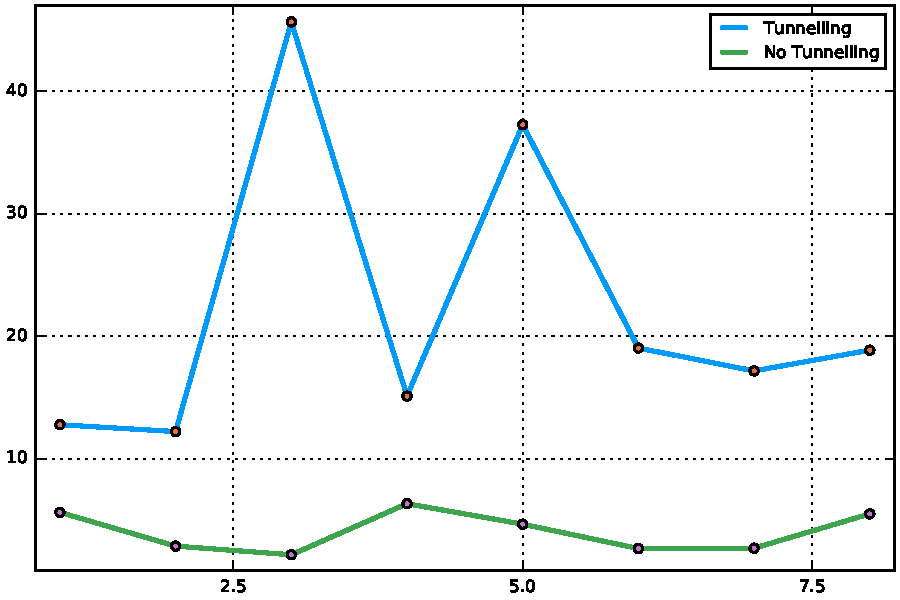
\includegraphics[scale=.5]{1.pdf}	
		\begin{tabular}{c|c|c}
		    & tunnel &  no tunnel \\ \hline
		1   & 12.786 ms&  5.631 ms\\
		2   & 12.225 ms&  2.875 ms\\
		3   & 45.676 ms&  2.167 ms\\
		4   & 15.123 ms&  6.334 ms\\
		5   & 37.285 ms&  4.665 ms\\
		6   & 19.046 ms&  2.674 ms\\
		7   & 17.179 ms&  2.705 ms\\
		8   & 18.874 ms&  5.505 ms\\
		\end{tabular}  
	\end{center}
	\textbf{Discussion:} using tunnel increase the ping number which is understandable because instead of directly transmit our UDP packets, we now need to transmit it through another intermediate server (i.e \texttt{tunneld}) which will increase time. \\

\noindent\texttt{traffic\_rcv/traffic\_snd:} \\
I sent 5 queries uing tunneling and not using tunneling. Below is the performance:
\begin{center}
	\begin{tabular}{c|c|c|c|c|c|c|}
	    & \multicolumn{3}{c|}{tunnel} & \multicolumn{3}{c}{no tunnel} \\ \hline
	    & Time & BPS&  PPS & Time & BPS&  PPS \\ \hline
	1   & 0.109  s& 7766275.5&  920  & 0.116 s& 7270135.5&  861 \\ 
	2   & 0.108  s& 7750229.5&  922& 0.108 s& 7767991.5&  920 \\ 
	3   & 0.108  s& 7784829  &  922& 0.109 s& 7675029.5&  909 \\ 
	4   & 0.108  s& 7781886  &  927& 0.107 s& 7855029.5&  929 \\ 
	5   & 0.109  s& 7731062  &  916& 0.119 s& 7061520.5&  836 \\ 
	\end{tabular}  	
\end{center}
\textbf{Discussion:} There are not many difference between using tunneling and not using tunneling because the throughtputs from \texttt{hicks libary} to \texttt{borg} and \texttt{sslab01} are similar. There will be no bottleneck node. Also, with tunneling, the result seems to be more stable at receiver, and I think the reason is that connection between \texttt{borg} machines and \texttt{sslab01} is more stable compared to connection between \texttt{hick} machine and \texttt{sslab} machines 
\end{problem}


\begin{problem}{2}
	
\end{problem}

\begin{problem}{3}
	Print and inspect all the fields of headers/trailers of the first three Ethernet frames, the headers of IP and UDP packets contained therein, and the first 10 bytes of the UDP payloads. The UDP header is very simple, containing 16-bit length and checksum fields in addition to source and destination port numbers. 
	\\
	Captured package: \\
	- First Package
	\begin{verbatim}
	    IP (tos 0x0, ttl 64, id 52721, offset 0, flags [none], proto UDP (17), length 4028)
	    192.168.1.2.35810 > 192.168.1.1.10000: UDP, length 4000
	    0x0000:  3a56 8f3e 2af8 babc 4274 5230 0800 4500  :V.>*...BtR0..E.
	    0x0010:  0fbc cdf1 0000 4011 19ec c0a8 0102 c0a8  ......@.........
	    0x0020:  0101 8be2 2710 0fa8 930d 4c4c 4c4c 4c4c  ....'.....LLLLLL
	    0x0030:  4c4c 4c4c 4c4c 4c4c 4c4c 4c4c 4c4c 4c4c  LLLLLLLLLLLLLLLL
	    0x0040:  4c4c 4c4c 4c4c 4c4c 4c4c 4c4c 4c4c 4c4c  LLLLLLLLLLLLLLLL
	\end{verbatim}
	- Second Package
	\begin{verbatim}
	    IP (tos 0x0, ttl 64, id 52722, offset 0, flags [none], proto UDP (17), length 4028)
	    192.168.1.2.35810 > 192.168.1.1.10000: UDP, length 4000
	    0x0000:  3a56 8f3e 2af8 babc 4274 5230 0800 4500  :V.>*...BtR0..E.
	    0x0010:  0fbc cdf2 0000 4011 19eb c0a8 0102 c0a8  ......@.........
	    0x0020:  0101 8be2 2710 0fa8 930d 4c4c 4c4c 4c4c  ....'.....LLLLLL
	    0x0030:  4c4c 4c4c 4c4c 4c4c 4c4c 4c4c 4c4c 4c4c  LLLLLLLLLLLLLLLL
	    0x0040:  4c4c 4c4c 4c4c 4c4c 4c4c 4c4c 4c4c 4c4c  LLLLLLLLLLLLLLLL		
	\end{verbatim}
	- Third package
	\begin{verbatim}
	    IP (tos 0x0, ttl 64, id 52723, offset 0, flags [none], proto UDP (17), length 4028)
	    192.168.1.2.35810 > 192.168.1.1.10000: UDP, length 4000
	    0x0000:  3a56 8f3e 2af8 babc 4274 5230 0800 4500  :V.>*...BtR0..E.
	    0x0010:  0fbc cdf3 0000 4011 19ea c0a8 0102 c0a8  ......@.........
	    0x0020:  0101 8be2 2710 0fa8 930d 4c4c 4c4c 4c4c  ....'.....LLLLLL
	    0x0030:  4c4c 4c4c 4c4c 4c4c 4c4c 4c4c 4c4c 4c4c  LLLLLLLLLLLLLLLL
	    0x0040:  4c4c 4c4c 4c4c 4c4c 4c4c 4c4c 4c4c 4c4c  LLLLLLLLLLLLLLLL	
	\end{verbatim}
	\begin{enumerate}
		\item 
		What is the default value of the TTL field observed?
		\\\textbf{Ans:} The default  TTL is 64
		\item Use the /bin/ping app to gauge the TTL values from www.purdue.edu, www.cisco.com, and another web site of your choice. 
		\\\textbf{Ans:} Using ping app, we get: \\
		\texttt{www.purdue.edu:} TTL = 250 
		\begin{verbatim}
		64 bytes from www.purdue.edu (128.210.7.200): icmp_seq=1 ttl=250 time=0.995 ms
		64 bytes from www.purdue.edu (128.210.7.200): icmp_seq=2 ttl=250 time=0.887 ms	
		\end{verbatim}
		\texttt{www.cisco.com:} TTL = 55 
		\begin{verbatim}
		a23-79-213-27.deploy.static.akamaitechnologies.com (23.79.213.27) ... ttl=55 ...
		a23-79-213-27.deploy.static.akamaitechnologies.com (23.79.213.27) ... ttl=55 ...
		\end{verbatim}
		\texttt{www.stackoverflow.com:} TTL = 57 
		\begin{verbatim}
		64 bytes from 151.101.129.69: icmp_seq=1 ttl=57 time=7.49 ms
		64 bytes from 151.101.129.69: icmp_seq=2 ttl=57 time=7.10 ms
		\end{verbatim}
		\item Do the values equal to the TTL value you observed during sniffing? 
		Check if TTL values can vary across operating systems and protocols. 
		\\ \textbf{Ans.} No. TTL during sniffing is 64 while other varies. Also, TTL values vary across OS and protocol. For example, in Windows 7, for IMCP/TCP/UDP, ttl is 128. In Linux/UNIX, TTL is 64 (may vary on different verions of Linux) 
		\item How might an attacker exploit TTL information from ping or other sources? 
		\\\textbf{Ans.} with knowledge of TTL information, adversary can send lots of packages in a way that those packages will expire at the switch/router. Thus, the switch is forced to generate large amount of ICMP exceed messages. This may caused heavy load on switch, and may cause Deny of Service on the target. 
		\item Is the TOS field being used in the sniffed IP packets?
		\\ \textbf{Ans.} No. In the sniffed IP package, the TOS field is after Version Number (i.e 4) and IFL (i.e 5), it's \texttt{00} which means it was not used.
 		\item How about the fragmentation fields?.
 		\\\textbf{Ans. }No. Because in our sniffed package, combination of flag field and fragmentation field  is \texttt{0000}. Therefore, framentation was not used.
	\end{enumerate}



\end{problem}

\end{document}
